\section{Financial\_\-Monthly\_\-Root  Class Reference}
\label{classFinancial__Monthly__Root}\index{Financial_Monthly_Root@{Financial\_\-Monthly\_\-Root}}
{\tt \#include $<$dil2al.hh$>$}

Inheritance diagram for Financial\_\-Monthly\_\-Root::\begin{figure}[H]
\begin{center}
\leavevmode
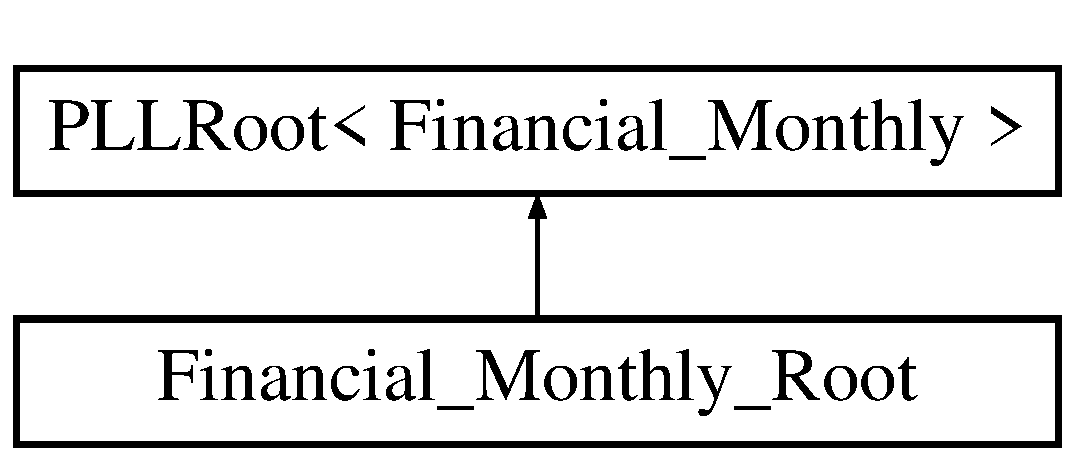
\includegraphics[height=2cm]{classFinancial__Monthly__Root}
\end{center}
\end{figure}
\subsection*{Public Methods}
\begin{CompactItemize}
\item 
{\bf Financial\_\-Monthly\_\-Root} ()
\item 
void {\bf add} (const {\bf Financial\_\-Note} \&fn)
\item 
{\bf String} {\bf put\_\-results} () const
\end{CompactItemize}


\subsection{Constructor \& Destructor Documentation}
\index{Financial_Monthly_Root@{Financial\_\-Monthly\_\-Root}!Financial_Monthly_Root@{Financial\_\-Monthly\_\-Root}}
\index{Financial_Monthly_Root@{Financial\_\-Monthly\_\-Root}!Financial_Monthly_Root@{Financial\_\-Monthly\_\-Root}}
\subsubsection{\setlength{\rightskip}{0pt plus 5cm}Financial\_\-Monthly\_\-Root::Financial\_\-Monthly\_\-Root ()\hspace{0.3cm}{\tt  [inline]}}\label{classFinancial__Monthly__Root_a0}




Definition at line 1148 of file dil2al.hh.



\footnotesize\begin{verbatim}1148 {};
\end{verbatim}\normalsize 


\subsection{Member Function Documentation}
\index{Financial_Monthly_Root@{Financial\_\-Monthly\_\-Root}!add@{add}}
\index{add@{add}!Financial_Monthly_Root@{Financial\_\-Monthly\_\-Root}}
\subsubsection{\setlength{\rightskip}{0pt plus 5cm}void Financial\_\-Monthly\_\-Root::add (const {\bf Financial\_\-Note} \& {\em fn})}\label{classFinancial__Monthly__Root_a1}




Definition at line 227 of file finances.cc.

References Financial\_\-Monthly::add(), Financial\_\-Monthly::Copy\_\-Categories(), Financial\_\-Note::Date(), Financial\_\-Monthly::Find\_\-Month(), PLLRoot$<$ Financial\_\-Monthly $>$::head(), PLLRoot$<$ Financial\_\-Monthly $>$::link\_\-before(), and time\_\-stamp().

Referenced by financial\_\-monthly().



\footnotesize\begin{verbatim}227                                                           {
228   // add by month
229   String mstr = time_stamp("%Y%m",fn.Date());
230   Financial_Monthly * fm = NULL;
231   if (head()) fm = head()->Find_Month(mstr);
232   if (!fm) { // add month
233       fm = new Financial_Monthly(mstr);
234       link_before(fm);
235       fm->Copy_Categories(head());
236   }
237   // check for new categories and subcategories
238   // add by category and subcategory within month
239   fm->add(fn);
240 }
\end{verbatim}\normalsize 
\index{Financial_Monthly_Root@{Financial\_\-Monthly\_\-Root}!put_results@{put\_\-results}}
\index{put_results@{put\_\-results}!Financial_Monthly_Root@{Financial\_\-Monthly\_\-Root}}
\subsubsection{\setlength{\rightskip}{0pt plus 5cm}{\bf String} Financial\_\-Monthly\_\-Root::put\_\-results () const}\label{classFinancial__Monthly__Root_a2}




Definition at line 242 of file finances.cc.

References PLLRoot$<$ Financial\_\-Monthly $>$::head(), PLL\_\-LOOP\_\-FORWARD, PLL\_\-LOOP\_\-FORWARD\_\-NESTED, and res.

Referenced by financial\_\-monthly().



\footnotesize\begin{verbatim}242                                                  {
243   String res;
244   PLL_LOOP_FORWARD_NESTED(Financial_Monthly,head(),1,m) { // month
245     res += "Month: " + m->Month() + '\n';
246     PLL_LOOP_FORWARD_NESTED(Financial_Monthly_Category,m->categories.head(),1,c) { // category
247       res += "<TABLE BORDER=1 WIDTH=\"100%\">\n<TR>";
248       // headings
249       PLL_LOOP_FORWARD(Financial_Monthly_SubCategory,c->subcategories.head(),1) { // subcategory
250         res += "<TH>" + e->SubCategory();
251       }
252       res += "<TH>" + c->Category() + "\n<TR>";
253       // results
254       PLL_LOOP_FORWARD(Financial_Monthly_SubCategory,c->subcategories.head(),1) { // subcategory
255         res += "<TD>" + String(e->Result(),"%.2f");
256       }
257       res += "<TH><B>" + String(c->Result(),"%.2f") + "</B>\n</TABLE>\n";
258     }
259   }
260   return res;
261 }
\end{verbatim}\normalsize 


The documentation for this class was generated from the following files:\begin{CompactItemize}
\item 
{\bf dil2al.hh}\item 
{\bf finances.cc}\end{CompactItemize}
